\documentclass{article}
\usepackage{graphicx}
\usepackage[utf8]{inputenc}

\title{Advances in Financial Machine Learning}
\author{M. Krishnamoorthy and S. Unger}
\date{\today}

\begin{document}

\maketitle
\tableofcontents 

\section{Part1:Data Analysis}
\subsection{Goal: }
-Learn how to produce matrix X of financial features out of an unstructured dataset. \\ 
-Unsupervised learning algorithms can learn the patterns from the matrix X(eg. whether it contains hierarchical cluster)

\subsection{Financial Data Structures}
- Describes how to work with unstructured financial data and from that to derive a structured dataset for Ml algorithms\\ 
- 4 essential types of Financial Data\\ 

\textbullet \textbf{Fundamental Data} (Assets, Liabilities, Sales, Cost/Earnings, Macro Variables)\\ 
-Fundamental data is extremely regularized and low frequency.  
It is rather unlikely that there is much value left to be exploited.  But may be useful in combination with other data types.\\ 

\textbullet\textbf{Market Data }( Price/Yield/Implied volatility, Volume, Dividend/coupons, Open interest.....)\\ 
- includes all trading activity that takes place in an exchange or trading venue\\ 
-  most likely data provider would have to provide the information such as FIX messages.....\\ 
-unlike Fundamental Data, this data is abundant with over 10TB generated daily\\ 

\textbullet \textbf{Analytics} (Analyst recommendations, Credit ratings, Earnings expectations, News sentiment)\\ 
-Could think of analytics as Derivate Data, based on an original source which could be Fundamental, Market, Alternative, or collection of other Analytics\\ 

\textbullet \textbf{Alternative Data }(Satellite/CCTV images, Google searches, Twitter/chats, Metadata)\\ 


\subsection{BARS}
\subsection{Standard Bars}
1)Time Bars\\ 
2)Tick Bars\\ 
3)Volume Bars\\ 
4)Dollar Bars\\ 

-Purpose of these methods is to transform a series of observations that arrive at irregular frequency("inhomogeneous series") into a homogeneous series derived from regular sampling \\ 

\textbullet \textbf{Time Bars} - are obtained by sampling information at fixed intervals(eg, once every minutes)\\ 
-(ex, Open Price, Close Price, High Price, Low Price)\\ 
-Although popular should be avoided because Markets do not process info at constant time interval and time sampled series often exhibit poor statistical properties(serial correlation, heteroscedasticity, non normality)\\ 

\textbullet\textbf{Tick bars}-idea behind it is that sample variables like (Open Price, Close Price, High Price, Low Price) will be extracted each time a pre-defined number of transactions take place(eg, 1000 tickets)\\ 
-"Price changes over a fixed number of transactions may have a Gaussian distribution. Price changes over a fixed time period may follow a stable Paretian distribution, whose variance is infinite."\\ 
-need to be aware of outliers\\ 
-Allows to synchronize sampling with a proxy of information arrival\\ 

\textbullet\textbf{Volume Bars}-Volume bars can sample every time a pre-defined amount of the securities units has been exchanged(ex, sample prices every time a futures contract exchanges 1000 units, regardless of the number of ticks involved\\ 
-(1973)Sample returns by volume achieved even better statistical properties than sampling by tick bars(i.e closer to an IID Gaussian distribution)\\ 

\textbullet\textbf{Dollar Bars}-formed by sampling an observation every time a pre-defined market value is exchanged.\\ 
"ex, suppose we wish to analyze a stock that has exhibited an appreciation of 100 percent over a certain period of time.  Selling 1000 worth of that stock at the end of the period requires trading half the number of shares it took to buy 1000 worth of that stock at the beginning.  The number of shares traded is a function of the actual value exchanged.\\ 
\subsection{Information Driven Bars}
-To sample more frequently when new information arrives \\ 
1)Tick Imbalance Bars\\ 
2)Volume/Dollar Imbalance Bars\\ 
3)TIBs, VIBs, DIBs(monitor order flow imbalance, as measure in terms of ticks, volumes, and dollar values exchanged)\\ 

\textbullet \textbf{Tick Imbalance Bars}\\ 
-We try to sample bars whenever tick imbalances exceed our expectation.\\ 
-Similar to STA457 project \\ 
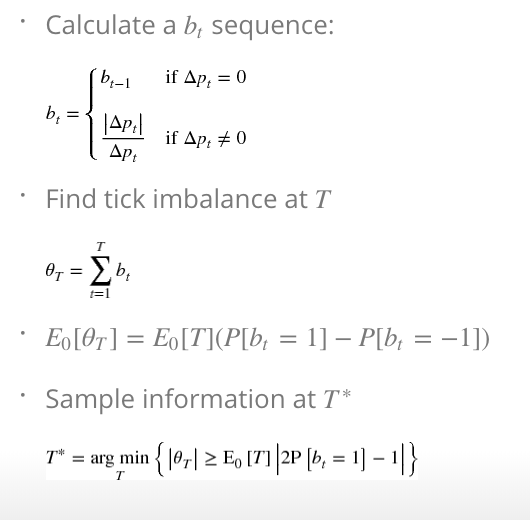
\includegraphics[width=\textwidth]{TickimbalanceBars.png}\\ 
-We try to determine the tick index, T, such that the accumulation of signed ticks exceeds a given threshold.\\ 
-Can't differentiate between order size of 10 and order 1(counts both as 1)\\ 

\subsection{More Information Driven bars:}
\textbullet \textbf{Volume/Dollar Imbalance Bars}\\ 
-The idea behind volume imbalance bars(VIB's) and dollar imbalance bars(DIBs) is we would like to sample bars when volume or dollar imbalances diverge from our expectations.\\ 
-TIBs, VIBs, DIBs monitor order flow imbalance as measures in terms of ticks, volumes, and dollar values exchanged.\\ 

\textbullet \textbf{Tick Runs Bars}\\ 
-Based on notions of tick rules and boundary condition discussed in TIBs, we can define a procedure to determine the index of the next sample, T.\\ 
-"Large traders will sweep the order books, use iceberg orders, or slick a parents order into multiple children, all of which leave a trace of runs in (bt) sequence"\\ 
-For that reason its better to monitor sequence of buys in the overall volume and take samples when that sequence diverges from our expectations.\\ 

\textbullet \textbf{Volume/Dollar Runs Bars}\\ 
-Volume Run Bar(VRBs), and Dollar Runs Bars(DRBs) \\ 
-We wish to sample bars whenever the volumes or dollars traded by one side exceed our expectation for a bar\\ 

\subsection{Dealing with Multi-Product Series\\ }
-interested in modelling a time series of instruments, where the weights need to be dynamically adjusted over time.\\ 
	\indent-other time we may deal with products that pay irregular coupons/dividends\\ 
-We will have structural breaks if time series that was altered by \\ 
\textbullet \textbf{The ETF Trick}(add more)\\ 
-we wish to develop a strategy that trades a spread of futures\\ 


\textbf{Nuisances}\\ 
-spread is characterized by a vector of weights that changes over time. \\ 
-As a result, the spread itself may converge even if prices do not change.(when that happens, a model trading that series will be misled to believe that PnL has resulted from that weight induced convergence)\\ 
-Spreads require negative values, b/c they do not represent a price\\ 

-Ways to avoid these issues is to produce time series that reflects the value of 1 Dollar invested in a spread.\\ 
-Changes in the series will reflect changes in PnL, the series will be strictly position and implementation shortfall will be taken into account.\\ 
-This series will be used to model, generate signals, and trade as if it were an ETF\\ 

\textbullet \textbf{PCA Weights}\\ 

\textbullet \textbf{Single Future Roll}\\ 
-When dealing with a single futures contract, an equivalent and more direct approach is to form a time series of cumulative roll gaps, and detract that gaps series from the prices series\\ 

\subsection{Sampling Features\\ }
-We learned how to produce a continuous, homogeneous and structured dataset from a collection of unstructured financial data\\ 
-Going to learn ways of sampling bars to produce a features matrix with relevant training examples.\\ 

\textbullet \textbf{Sampling for Reduction}\\ 
-Sampling features from dataset to reduce the amount of data used to fit the ML algorithm\\ 

\textbullet \textbf{Event-Based Sampling} - CUSUM Filter \\ 
-The CUSUM filter is a quality control method, designed to detect a shift in the mean value of a measure quantity away from a target value\\ 

\section{Labeling}
\subsection{Goal:\\ }
-Describes ways to label financial data\\ 
-Supervised learning algorithms require that the rows of X are associated with an array of labels/values y, so that those labels/values can be predicted on unseen features samples\\ 
-create response variables for supervised learning\\ 

\subsection{The Fixed Time Horizon Method}\\ 
-Almost all ML papers label observations using the fixed time horizon method\\ 
-Features matrix X with I rows, each row (Xi) is the features sampled from some bars with index t=1,…,T, where  I≤T\\ 
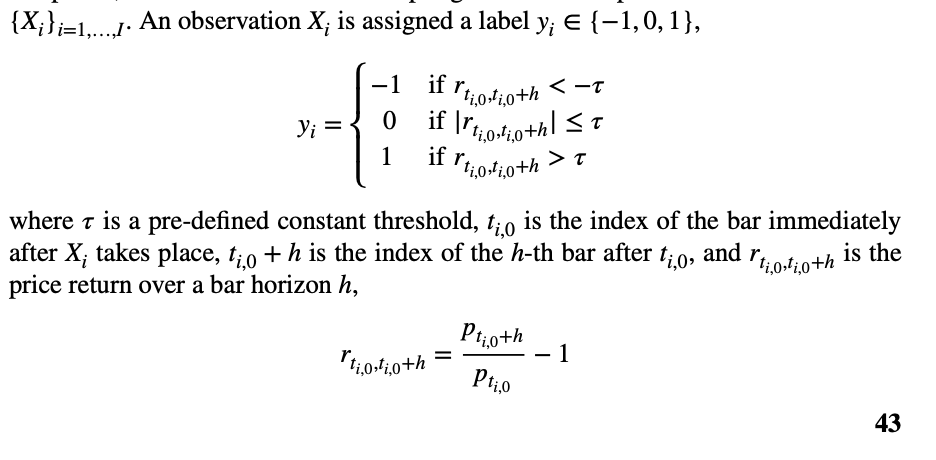
\includegraphics[width=\textwidth]{FixedHorizonMethod.png}\\ 
-For each Xi(row vector), we assign label yi\\ 
-Features = Independent variables/predictors;\\ 
-Label = response variable \\ 
-Limitations:\\ 
	\indent-h is fixed and time bars do not exhibit good statistical properties \\ 
    \indent-the threshold of tau is fixed regardless of the observed volatility\\ 
Alternatives:\\ 
	\indent1)Label per a varying threshold (sdt), estimated using a rolling 				  		exponentially weighted standard deviation of returns\\ 
    \indent2)Use volume/dollar bars, as their volatility's are much closer to constant(homoscedasticity)\\ 
    \indent Even these 2 improvements don't improve the flaw: path followed by 		    	prices\\ 
 \indent Stop Loss limits ???  \\ 
 
\subsection{Computing Dynamic Thresholds}\\ 
-In practise we want to set profit taking and stop loss limits that are a function of the risks involved in a bet\\ 
-Run R code"Daily Volatility Estimates"\\ 

\subsection{The Triple Barrier Method}\\ 
-Labels an observation according to the first barrier touched out of three barriers\\ 
		\indent1)we set 2 horizontal barriers, and 1 vertical barrier\\ 
    	\indent2)The horizontal barriers are defined by profit taking, and stop loss  	  				limits, which are a dynamic function of estimated volatility\\ 
        \indent3)the third barrier is defined in terms of the number of bars elapsed since 		the position was taken(an expiration limit)\\ 
        \indent4)If upper barrier is touched first, we label observation as 1\\ 
        \indent5)If the lower barrier is touched first, we label the observation as -1\\ 
        \indent6)If the vertical barrier is touched first, we have two choices: the sign of 
        the return, or a 0(Author prefers sign of return as a matter of realizing a 		profit or loss within limits)\\ 
-Triple barrier method is path dependent(?)\\ 
-[pt, sl, t1]\\ 
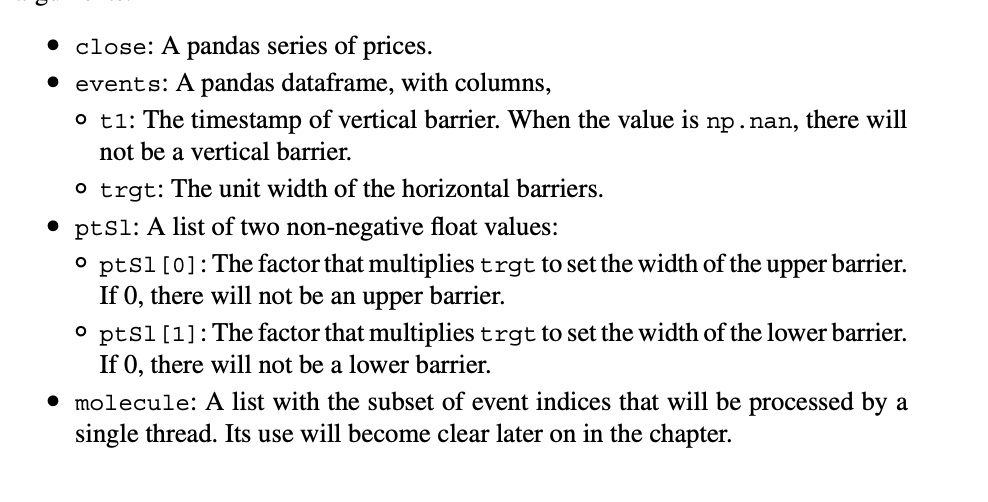
\includegraphics[width=\textwidth]{abv.png}\\ 
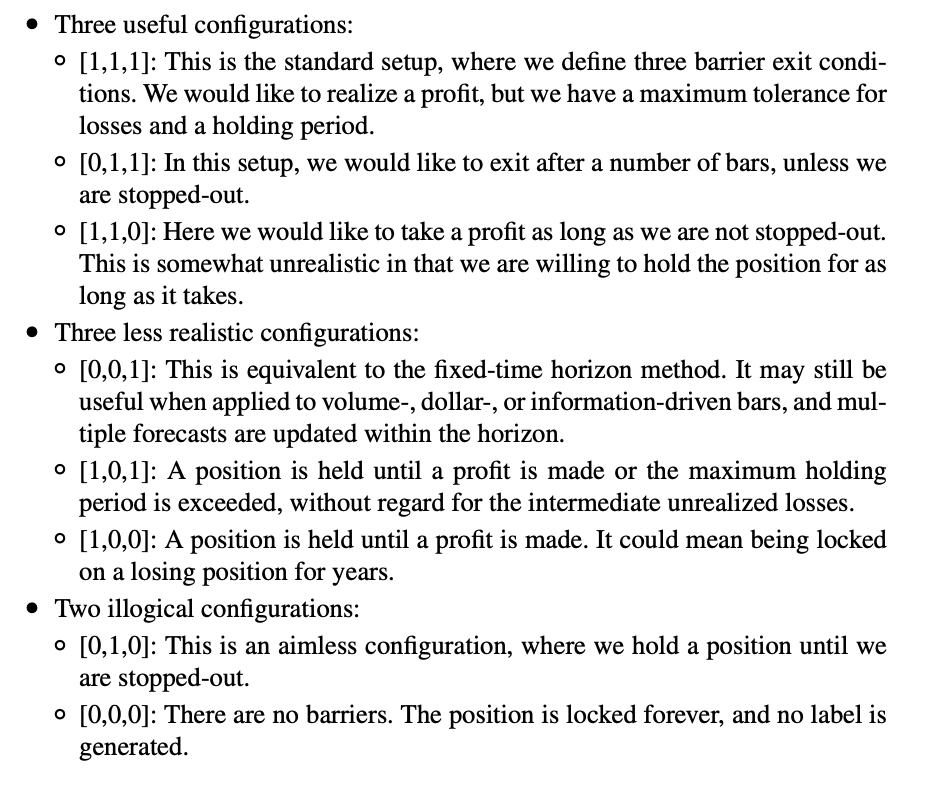
\includegraphics[width=\textwidth]{TripleBarrierMethod.png}\\ 
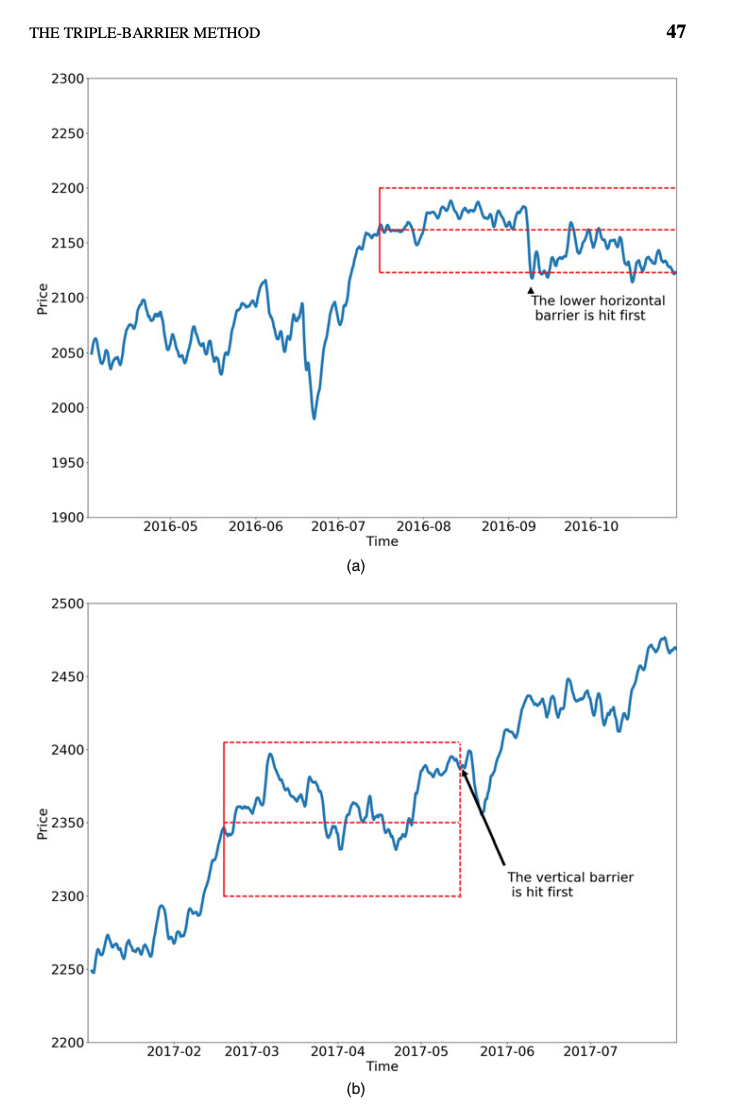
\includegraphics[width=\textwidth]{TriplePicture.png}\\

\subsection{Learning Side and Size}\\ 
-learn how to label examples so that an ML algorithm can learn both the side and the size of a bet\\ 
	\indent-interested in learning the side of a bet when we do not have an \textbf{underlying model} to set the sign of our position(long or short)\\ 
-under that circumstance, we cant differentiate between a profit taking barrier, and a stop loss barrier, since it requires knowledge of the side\\ 
-Learning size implies that either there are no horizontal barriers or that the horizontal barriers must be symmetric\\ 

\subsection{Meta Labeling}\\ 
-Learn what is the appropriate size of the bet \\ 
		\indent-We already have a model for setting the side of the bet(long, short)\\ 
       	\indent-Now we need to learn the size of the bet, which includes the possibility 			of no bet at all(zero size)\\ 
       \indent -We often know whether we want to buy or sell a products, only 						remaining question is how much money we should risk in such a bet.\\ 
        \indent-Don't want Ml algorithm to learn the side, just want it to tell us what is 			appropriate size\\ 
- **Make some adjustments to previous code in order to handle meta labeling(look at code that expands getEvents to incorporate Meta-Labeling)\\ 
-Primary model: learning only the side of the best(eg, moving average crossing strategy)\\ 
-Quantamental investment research\\ 

\textbf{How to use Meta-Labeling?}\\ 
-Meta-Labeling is helpful when you want to achieve highest F1 scores.\\ 
		\indent-\textbf{F1 Scores}:measures the efficiency of a classifier as the harmonic average between precision and recall???\\ 
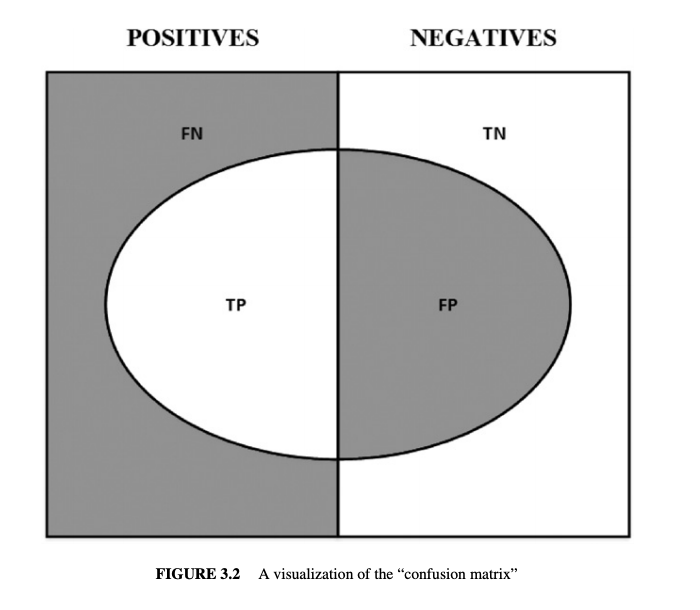
\includegraphics[width=\textwidth]{Confusion.png}\\ 
		\indent-Binary Classifier predicts that some items exhibit the condition (ellipse), 		 where the TP area contains the true positives and TN are contains the true negatives\\ 
        \indent-Leads to 2 kind of erros:False Positives(FP), and False Negatives(FN)\\ 
        \indent-Precision is the ratio between TP area and the area in the ellipse.\\ 
        -Recall is the ratio between the TP area and the area in the left rectangle\\ 
		\indent-Accuracy is the sum of the TP and TN areas divided by the overall set of
        items(square)\\ 
        \indent-decreasing the FP are comes at a cost of increasing the FN area, because 			higher precision typically means fewer calls, hence lower recall.\\ 
        \indent-There is some combination of precision and recall that maximizes the 
        overall efficiency of the classifier.\\ 
1) we want to build model that achieves high recall, even if the precision is not particularly high\\ 
2) we correct for the low precision by applying meta-labeling to the positives predicted by the primary model\\ 
	\indent-Meta-Labeling will increase your F! score by filtering out the false 					positives, where the majority of positives have already been identified by 	the primary model\\ 
    
\textbf{Reasons why Meta-Labeling is powerful}\\ 
1)Since ML algorithms are criticized as black boxes, Meta-Labeling allowed you to build an ML system on top of a white box(like a fundamental model founded on economic theory)\\ 
	\indent-ability to transform a fundamental model into an ML model makes meta-		labeling useful\\ 
2)Effects of over fitting are limited when you apply meta-labeling, because ML will not decide the side of your bet, only the size\\ 
3)By decoupling the side prediction from the size prediction, meta-labeling enables sophisticated strategy structures(eg, features driving a rally may differ from the features driving a sell off, in that case you want to develop an Ml strategy exclusively for long positions, based on the buy recommendations of a primary model, and an ML strategy exclusively for short positions, based on the sell recommendations of an entirely different primary model)\\ 
4)Achieving high accuracy on small bets and low accuracy on large bets are disastrous.\\ 
-Makes sense to develop an ML algorithm solely focused on getting the sizing right(equally as important as identifying good opportunities)\\ 

\textbullet\textbf{The Quantamental Way}\\ 
-High demand among hedge funds for technologies that combine human expertise with quantitative methods\\ 
-Can add meta-labeling layer to any primary model, whether that is an ML algorithm, an econometric equation, technical trading rule, or a fundamental analysis.\\ 
ex, the meta-labeling ML algorithm could find that discretionary Portfolio Managers tend to make particularly good calls when there is a structural break, as they may be quicker to grasp a change in market regime, or another ex, it may be that PM's under stress, as evidenced by few hours of sleep, fatigue, change is weight tend to make inaccurate predictions. \\ 


\end{document}
